\chapter{Introduction}
Lorem ipsum dolor sit amet, consetetur sadipscing elitr, sed diam nonumy eirmod tempor invidunt ut labore et dolore magna aliquyam erat, sed diam voluptua. At vero eos et accusam et justo duo dolores et ea rebum. \cite{Abedon2003}

{\color{red}some colored text}

\section{First Section}
Lorem ipsum dolor sit amet, consetetur sadipscing elitr, sed diam nonumy eirmod tempor invidunt ut labore et dolore magna aliquyam erat, sed diam voluptua. At vero eos et accusam et justo duo dolores et ea rebum. Stet clita kasd gubergren, no sea takimata sanctus est Lorem ipsum dolor sit amet. Lorem ipsum dolor sit amet, consetetur sadipscing elitr, sed diam nonumy eirmod tempor invidunt ut labore et dolore magna aliquyam erat, sed diam voluptua. At vero eos et accusam et justo duo dolores et ea rebum. Stet clita kasd gubergren, no sea takimata sanctus est Lorem ipsum dolor sit amet. \cite{Goossens1993}

\section{Embedding code samples}
Code listings can be modified with \textbackslash lstset (see .sty file). Code samples can either be embedded directly inline, as displayed in listing \ref{lst:python_inline_sample}.
% Also see: https://en.wikibooks.org/wiki/LaTeX/Source_Code_Listings.

%\begin{minipage}{\linewidth}
\begin{lstlisting}[caption={Python hello function.},captionpos=b,language=python,label=lst:python_inline_sample]
# prints hello
def hello(name):
    print('Hello, {}'.format(name))
\end{lstlisting}
%\end{minipage}
%
Or by including a file like so, see \ref{lst:python_file_sample}. To avoid page breaks within code snippets, use the minipage environment. This also smallers the code area which means it's aligning the line numbers with the "normal" text.

%\begin{minipage}{\linewidth}
\lstinputlisting[caption={Python hey function.},captionpos=b,label=lst:python_file_sample,language=python]{src/sample.py}
%\end{minipage}

\section{Images and labeling}
In order to include images, you need the graphicx package. The environment \textbackslash begin\{figure\} allows to label images. \textbackslash centering centers the image horizontally. \textbackslash includegraphics embeds the image (see figure \ref{fig:lighthouse}). 

\begin{figure}[h]
\centering
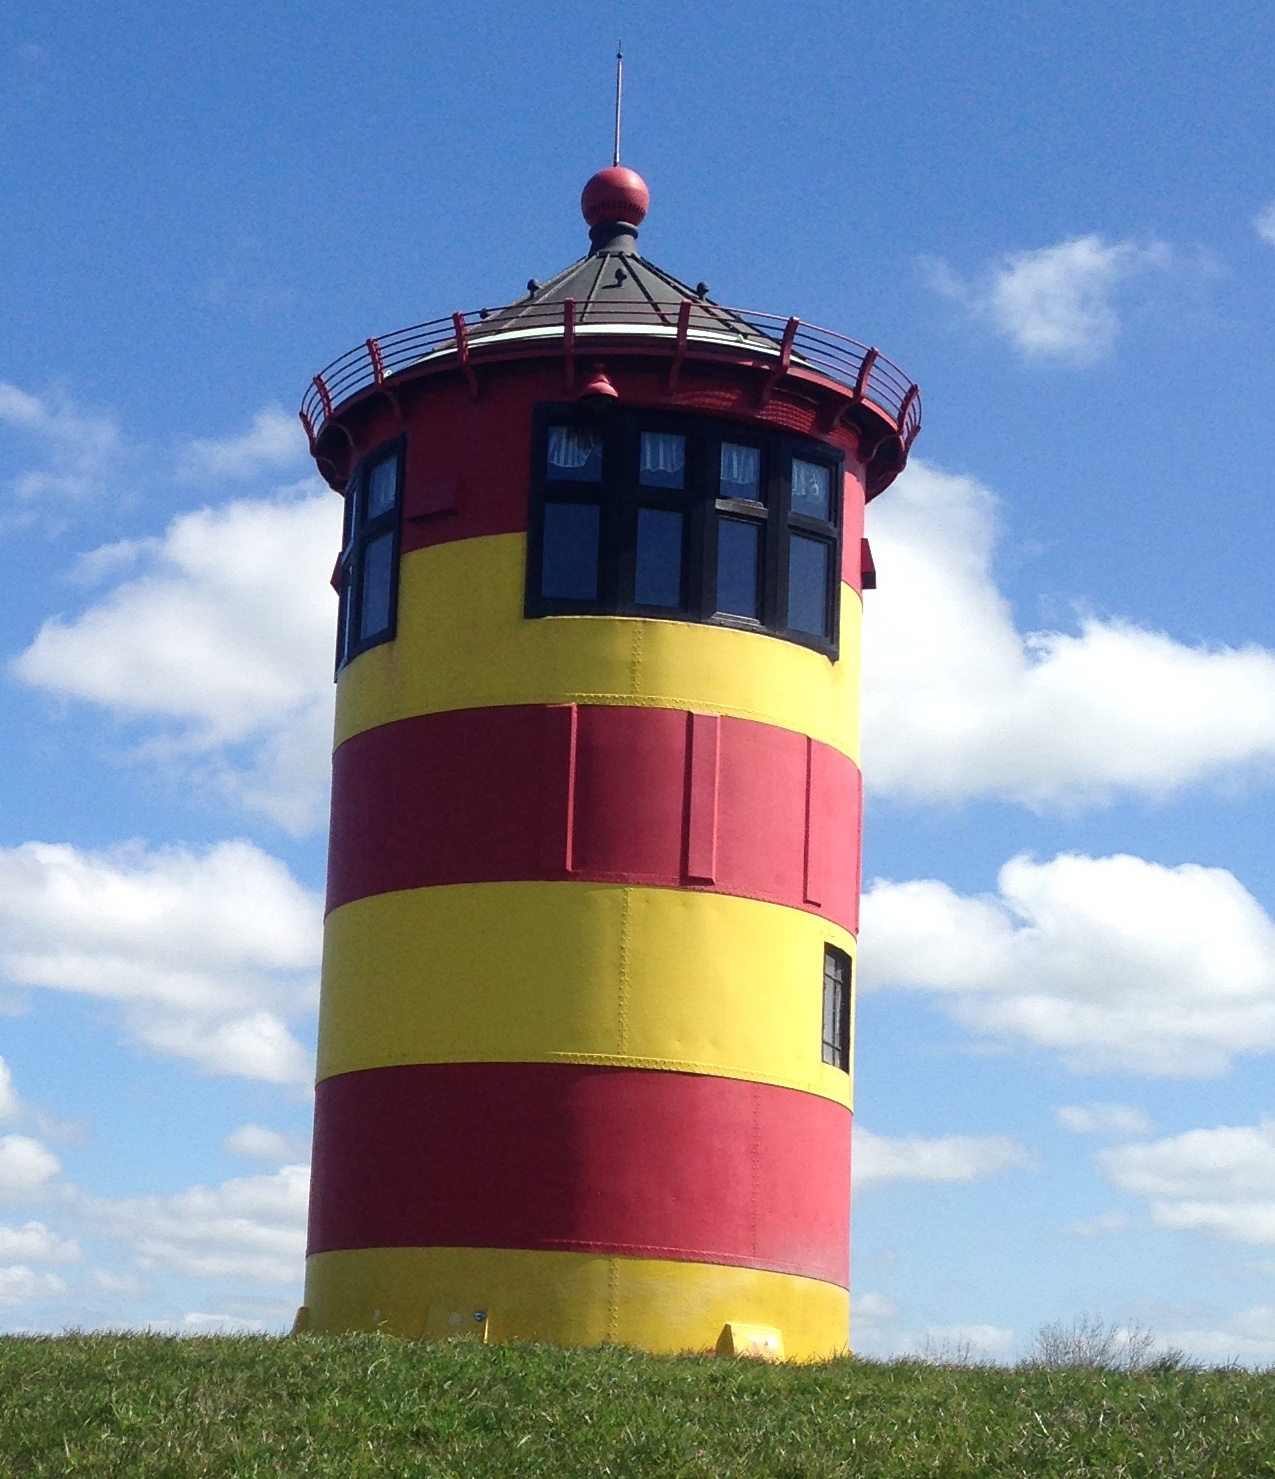
\includegraphics[width=0.5\textwidth]{img/lighthouse.jpg}
\caption{A red and yellow lighthouse.}
\label{fig:lighthouse}
\end{figure}














